\section{Introduction}
Wupper \footnote{A wupper is a person performing the act of bongelwuppen, the version from the Dutch province of Groningen of the Frisian sport Fierljeppen (canal pole vaulting). \href{https://www.youtube.com/watch?v=Bre8DsQZqSs}{https://www.youtube.com/watch?v=Bre8DsQZqSs}} was designed for the ATLAS / FELIX project \cite{atlas}, to provide a simple
Direct Memory Access (DMA) interface for the Xilinx  Virtex-7 PCIe Gen3 hard block and the . The core is not meant to be flexible among different architectures, but especially designed for the 256 bit wide AXI4-Stream interface
\cite{ug761}  of the Xilinx Virtex-7 and Ultrascale FPGA Gen3 Integrated Block for PCI Express (PCIe) \cite{xilinxcore}
\cite{pg023} \cite{pg156}. 

The purpose of the PCIe Engine is to provide an interface to a standard FIFO. This FIFO has the same width as the Xilinx AXI4-Stream interface (256 bits) and runs at 250 MHz. The application side of the FPGA design can simply read or write to the FIFO; the PCIe Engine will handle the transfer into Host PC memory, according to the addresses specified in the DMA descriptors.

With the PCIe Gen3 standard it is possible to reach a theoretical line rate of 8 GT/s; by using 8 lanes, it is therefore possible to reach a theoretical throughput of 64 Gb/s.
The main purpose of Wupper is to handle data transfers from a simple user interface, i.e a FIFO, to and from the host PC memory. The other functionality supported by Wupper is the access to control and monitor registers inside the FPGA, and the surrounding electronics, via a simple register map. Figure~\ref{fig:simplewupperpackage1} below shows a block diagram of the Wupper package.
 
\begin{figure}[h]
	\centering
	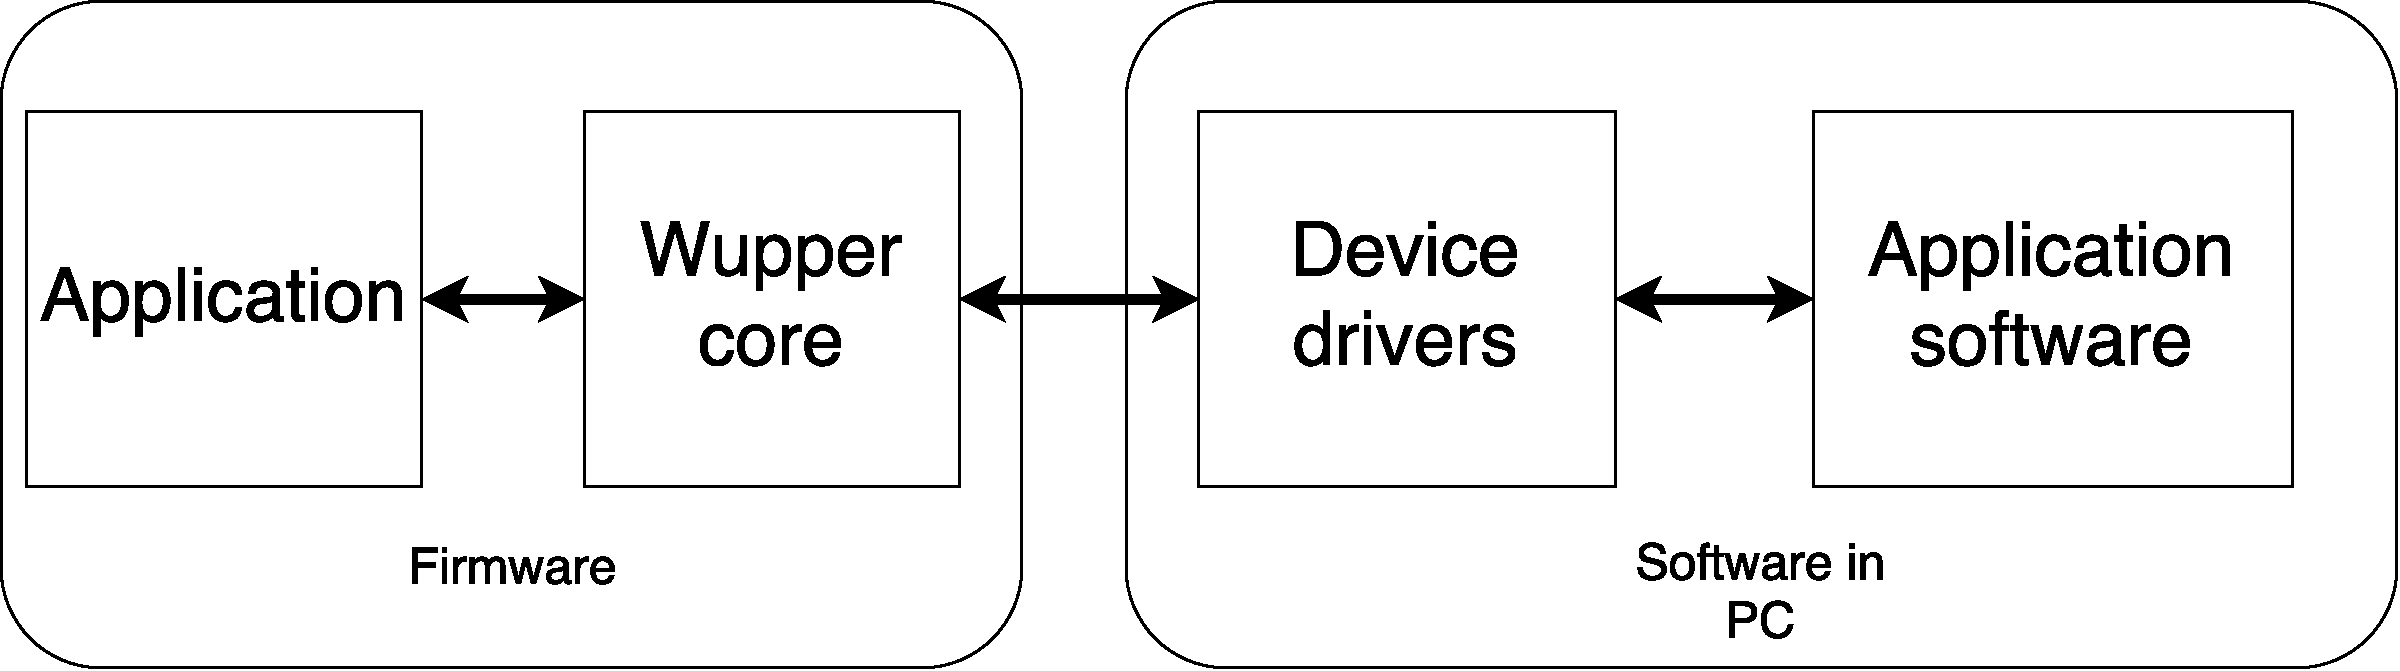
\includegraphics[width = .8 \textwidth]{figures/wupper_package_simple.pdf}	
	\caption{Wupper package overview}
	\label{fig:simplewupperpackage1}
\end{figure}
The Wupper core communicates to the host PC via the Wupper driver and is controlled by a set of, so called, Wupper tools. The Wupper driver through an Application Programming Interface (API) can also communicate to a Wupper Graphical User Interface (GUI). Wupper had been published under the LGPL license on Opencores.org~\cite{opencores}. As the developers firmly believe in the dissemination of knowledge through Open Source. Hence users can freely download, use and learn from the core and possibly provide feedback to further improve Wupper. The outcome of the development is the so called Wupper package: a suite of firmware and software components, which details will be given later in this report. On missing feature of the Wupper core published on OpenCores was a simple yet complete example application to study, test, and benchmark Wupper. To avoid confusion concerning name, a list is created to specify a name and description for all the parts of the Wupper project:

\begin{itemize}
	\item Wupper core: firmware PCIe engine
	\item Wupper driver: software device driver
	\item Wupper tools: software tools to operate the core
	\item Wupper GUI: a simple control and monitor panel
	\item Wupper package: the sum of the above packed for distribution on Open Cores.
\end{itemize}

For synthesis and implementation of the cores, it is recommend to use Xilinx Vivado 2015.4. The cores (FIFO, clock wizard and PCIe) are provided in the Xilinx .xci format, as well as the constraints file (.xdc) is in the Vivado 2015.4 Format.

For portability reasons, no Xilinx project files will be supplied with the Engine, but a bundle of TCL scripts has been supplied to create a project and import all necessary files, as well as to do the synthesis and implementation. These scripts will be described later in this document.


\newpage